% The entire content of this work (including the source code
% for TeX files and the generated PDF documents) by 
% Hongxiang Chen (nicknamed we.taper, or just Taper) is
% licensed under a 
% Creative Commons Attribution-NonCommercial-ShareAlike 4.0 
% International License (Link to the complete license text:
% http://creativecommons.org/licenses/by-nc-sa/4.0/).
\documentclass{article}

\usepackage{float}  % For H in figures
\usepackage{amsmath, amssymb} % For math
\usepackage{mathtools} % dcases*, see https://en.wikibooks.org/wiki/LaTeX/Advanced_Mathematics#The_cases_environment
\numberwithin{equation}{subsection} % have the enumeration go to the subsection level.
									% See:https://en.wikibooks.org/wiki/LaTeX/Advanced_Mathematics
\usepackage{graphicx}   % need for figures
\usepackage{cite} % For bibligraphy
\usepackage{fancyref} % For lazy reference \fref
\usepackage{hyperref} % For hyperlink everything.
\usepackage{CJKutf8} % For Chinese characters
%\usepackage{ dsfont } % For double struck fonts
\usepackage{braket} 
\usepackage[T1]{fontenc}
\usepackage{listings}

\usepackage{amsthm}
\newtheorem{defi}{Definition}[section]
\newtheorem{thm}{Theorem}[section]
\newtheorem{lemma}{Lemma}[section]
\newtheorem{remark}{Remark}[section]
\newtheorem{prop}{Proposition}[section]
\newtheorem{coro}{Corollary}[section]
\theoremstyle{definition}
\newtheorem{ex}{Example}[section]


\title{Draft}
\date{\today}
\author{we.taper}
\begin{document}
\maketitle
\abstract{
    This is a draft.
}
\tableofcontents

\section{Lectures on the Frontiers of Physics}
\textbf{Given by professor of physics in SUSTC}
    \subsection{By JQ. He.}
    \textbf{Thermal electrics}

    \subsection{By Lang. Chen}
    \label{sec:c.l}
    Grow thin films.
    \begin{itemize}
	\item Rheed-Assited PLD/MBE. (Ray as an exmination).
	\item 
	orbital contral of electrons -> 
	orbitronics -> Control of Spin orbital coupling.
	\item
	Multiferroics -> multiple order parameters, and the interaction
	between them. E.g. $BiFeO_3$.
	\item
	Ferrotorodicity: Spontaneous Toroidal Momennt. Time and spacial
	symmetries simultaneous broken.
	\item
	What is a iridates $Ir_2(X)O_4$, (e.g. $Sr_2RuO_4$) 
	exactly in theoretical physics?
	\item
	$H_2S$: 200K superconductor?
	\item
	The Double Exchange effect of oxygem -> Half-metal, phase transition.
    \end{itemize}

    \subsection{By Alan}
    \textbf{Photocatalysis}: $TiO_2$. Hongkong has $TiO_2$ spurred on
    the keys.

    \subsection{By Li, Huang}
    \begin{itemize}
            \item Computational Physics
            \item Surface Dynamics
            \item Structural factor from 2D to 3D.
            \item Finding Order Amid the Chaos. amorphous -> spatially
                    resolved distributed function.
            \item ?: What is genetically algorithm.
    \end{itemize}
    \textbf{Computational and theoretical studies of Surface dynamics}
    
    \begin{itemize}
            \item Surface atoms is immersed in a very different environment
                    compared with the bulk atoms.
            \item First-principle calculations
            \item DFT + LDA -> Conser equation
            \item Plane wave basis + Ultrasoft pseudopotentials to solve the
                    Conser equation
            \item Continumm method ?
    \end{itemize}

    \subsection{By Junfen, Liu}
    \begin{itemize}
            \item electronic transport in mesoscopic systems:
            \item Spintronics
            \item Graphene eletronics
            \item Superconductors etc.
    \end{itemize}
    \textbf{Quantum wire conductiing}
    The conduction channel in quantum wire is quantized, with discrete value
    of conductance.
    \begin{itemize}
            \item $\lambda_F$ Fermi wavelength
            \item $L_m$ Momuntum relaxation length <-- impurities.
            \item $L_\phi$ Phase relaxation length <-- memory of phase,
                    related to energy $\omega = E/\hbar$.
            \item $L$ Sample length
    \end{itemize}
    \begin{itemize}
            \item Ballistic transport: $L << L_m$ No scattering.
            \item Diffusive $L>L_m$, scattering, reduced transmission.
            \item Localization $L_m<<L<<L_\phi$ -> Prof. Haizhou Lu.
            \item Classical. (Omitted)
    \end{itemize}
    \textbf{Conductance}
    No back-scattering $$ G = \frac{I}{V} = \frac{2e^2}{h}$$
    Landauer formula $G = \frac{2e^2}{h}\cdot T$, $T$ is some coefficient
    accounting for the back scattering, perhaps the transmission
    probability.
    In reality, $G=\sum_{\text{Different channels}}G_i$, 

    We can turn the $G$ into resisivity: 
    $$\text{Resistance}= \frac{h}{2e^2} + \frac{h}{2*e^2}\frac{R}{T}$$
    $R+T=1$

    \paragraph{Resonate Transmission} (Omitted)

    \paragraph{Spintronics} Use the extra freedom of Spin. 
    
    Spin field eletroncis: Datta and Das, Appl. Phys. Lett. 56, 665(1990)

    GMR: 2007 Nobel prize in Physics.
    
    Hall Effect (Omitted)
    Spin Hall Effect: S. murakami, et.al. Science 301 1348(2004);
    

    J. Sinova et.al. Phys.Rev.Lett. 92, 126603 (2004). (Omitted)
    
    \paragraph{Graphene} Carrier -> Relativistic Dirac fermions.
    \textbf{Klein Paradox} 

    \paragraph{Josephson Junction} A phase difference could conduct
    electricity in Superconductors.
    


    \subsection{By Haizhou, Lu}
    \paragraph{Quantum Anomalous Hall Effect}
    Requires strong magnetic field: $\approx 10$ Tesla.

    Anomalous Hall Effect: Without magnetic field. $R_H = R_0 B+ R_A M$
    where $M$ is the magnetic susceptibility.
    Two-factors: SO coupling. Spin-dependent Hall Effect.
    
    An excellent illustrations is found in \cite{Arxiv-Xiao}:
    \begin{figure}[H]
        \centering
        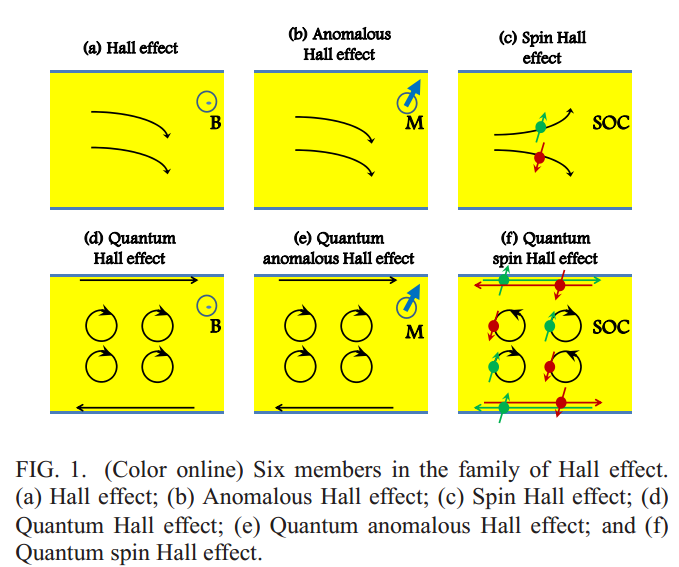
\includegraphics[width=0.8\linewidth]{pics/1}
        \caption{Illustration}
        \label{fig:Xiao Illustration}
    \end{figure}

    \subsection{By Kedong Wang}
    Tunneling current $I\propto V e^{-2kz}$, where 
    $k = \frac{\sqrt{2m\phi}}{\hbar}$, $\phi$ is the Work function.
    $I$ is very sensitive to the distance $z$.
    
    \paragraph{Work function} $\phi$ characterize the obstruction
    that prevents electron from escaping the sample.

    \subsection{By Mingyuan Hunag}
    Too boring.
    
    \subsection{By Wenkang Wong}
    \paragraph{Non-clone Theorem} We can easily see that there is no universal
    copy operators in Quantum Mechanics.

    \begin{proof}
    We proove it by contradiction. Let $U$ be the copy operator. By definition,
    we have
    $$   U \ket{\psi}\ket{0} = \ket{\psi}\ket{\psi}$$
    For any $\ket{\psi}$.
    Then, let try copying the state $\ket{\psi} = \ket{0} + \ket{1}$. We have
    \begin{align*}
        (\ket{0}+\ket{1})(\ket{0}+\ket{1}) &= U (\ket{0}+\ket{1})\ket{0} \\
        &= U (\ket{0}\ket{0} + \ket{1}\ket{0} ) \\
        &= \ket{0}\ket{0} + \ket{1}\ket{1} \\
    \end{align*}
    This is a contradiction.
    \end{proof}
    \begin{remark}
        We assume that the copyer is universal. This might seems to be too
        strong. However, if we assume that the copyer only
        works for certain states $\ket{\phi}$, then with the knowledge
        of these certain states, we could in principle create an exact copy
        of these states. This copy ,in the sense of another instance of the
        same object, of original state should not be considered to be an
        copied version of the original state.
    \end{remark}
    
\section{Problems in Bernevig's Topological ...}

    \subsection{Chapter 2}
    \paragraph{Non-Abelian Berry Transport}
    Derive Berry curvature to the adiabatic transport of a degenerate
    multiplet of states separated by a gap from the excited states.
    (Cautious about rotation within degenerate states).

    Answer: $\gamma_{mn}(t) = i \int_0^t \braket{m(R(t'))|\frac{d}{dt'}|n(R(t'))}dt'$

    Approach:
    Assuming that the those degenerate states are labeled by $1\cdots N$. 
    Thus we have naturally:
	\begin{align}
            H\phi &=i\hbar\frac{\partial}{\partial t}\phi\text{,  }
        \phi = \sum_n A_n \psi_n
    \end{align}
    
    Then we have:
    \begin{align}
    H \sum_n A_n \psi_n &=i\hbar\frac{\partial }{\partial t}
	  	\sum_n A_n(t) \psi_n(R(t)) \nonumber\\
	\sum_n E A_n \psi_n&=i\hbar\sum_n
		\left(
		\frac{\partial A_n(t)}{\partial t}\psi_n(R(t))+
		A_n(t)\frac{\partial \psi_n(R(t))}{\partial t}
		\right) \nonumber\\
	E A_m &=i\hbar
		\frac{\partial A_m(t)}{\partial t}
		+\sum_n A_n(t)\braket{m|\frac{\partial }{\partial t}|n}
    \end{align}
    Put in another form:
    $$
    \sum_n \left(\delta^n_m E
        - \braket{m| \frac{\partial}{\partial t}|n} \right) A_n
        =
    i\hbar \frac{\partial A_m(t)}{\partial t}
    $$
    In matrix form:
    \begin{align}
            (E - P) \mathbf{A} = i\hbar \dot{\mathbf{A}}
    \end{align}
    where:
    \begin{align}
        E &= \left(
        \begin{array}{ccc}
         \cdots   &     &   \\
              & E &   \\
             &    & \text{...} \\
        \end{array}
        \right) \\
        P &= (P^m_n) = \left(
        \braket{m| \frac{\partial}{\partial t}|n}\right)\\
        A &= \left(\begin{array}{c}
            A_1(t) \\
            A_2(t) \\
            \cdots \\
        \end{array}\right)
    \end{align}
    
    Note that $\braket{n| \frac{\partial}{\partial t}|m}^* \neq
    \braket{m| \frac{\partial}{\partial t} |n}$, thus $P$ may not be
    Hermitian.Ergo $E-P$ is Hermitian. So it is diagonalizable.

    Notice that
    \begin{align}
            0= \frac{\partial}{\partial t} \braket{m|n} &=
        \braket{\frac{\partial}{\partial t}m|n} +
        \braket{m|\frac{\partial}{\partial t}n} &&(\text{any }m,n)
    \end{align}
    temporary mathematica code:

% In[8]:=DSolve[{y1'[x]+y2'[x]==x,y1'[x]-y2'[x]==0},
%         {y1[x], y2[x]}, x]
% In[9]:= DSolve[{e1*A1[t]==A1'[t]+A1[t]*m1+A2[t]*m2, 
% e1*A2[t]==A2'[t]+A1[t]*m1+A2[t]*m2},{A1[t],A2[t]},t]
% In[10]:=DSolve[{e1*A1[t]==A1'[t]+A1[t]*m1},{A1[t]},t]
    

\section{Miscellnaneous Notes}
    \subsection{Super conductor}
    Mean-field approach to deal with a four operator diagonalization.
    
    Suppose we have: $D^*C^* CD$, then let $\delta = CD - \braket{CD} =
    CD - avg$. Then if we assume $\braket{CD}\neq 0$, and $\delta \approx 0$. Then we have:
    
    	$$ \delta^2 \approx 0 $$
    i.e.:
    
    \begin{align}
    	( (CD)^* - avg ) ( CD - avg ) = 0\\
    	D^*C^*CD = avg*(CD+D^*C^*) - avg^2
    \end{align}
    Hence a four operator is reduced into a few of two operators.
    Such method could be naturally extended to treat the operator
    $\sum_{i,j} D^*_i C^*_i C_j D_j$.
    
    A copper pair has the energy of:
    $$\Delta = \braket{C_{k \uparrow}C_{-k \downarrow} }$$
    
    To resist the flow of current carried by Copper Pair, is equivlant to destroying a pair of Copper Pair:
    $$ \braket{C_{k \uparrow}C_{-k \downarrow} } \longrightarrow C_{k \uparrow}C_{-k \downarrow}$$
    
    This will require an additional enegy of $2\Delta$.
    
    The exact meaning of "equivalent to" is as follows:
    \begin{align}
        & \text{break a copper pair} \longrightarrow 
        \text{scatter two electrons consecutively} 
        \nonumber\\ & \longrightarrow 
        \text{create two electron-hole mixed type quasi-particle} \longrightarrow 2\Delta \nonumber
    \end{align}

    \subsection{Why 0/0 is undefined?}
    If we suppose
    $$ \frac{0}{0}= \triangle $$
    Consider the following derivation:
    \begin{align}
	    \frac{0}{0} \cdot 1 &= \triangle \cdot 1 = \triangle \\
	    0 \cdot \frac{1}{0} &= \triangle\\
	    \Rightarrow \triangle &= 0
    \end{align}
    This is already bad enough. And we are forced to define $\frac{1}{0}$.
    Let $\frac{1}{0} = \square$, which literally means $1=0\cdot \square = 0$.
    This is disastrous.

    Alternatively, we could let
    \begin{enumerate}
	    \item Let $\frac{1}{0}$ be undefined.
	    \item Or let $\frac{1}{0} =
		    \infty$.
	    \item Or, let $\frac{a}{b}\cdot c= a\cdot \frac{c}{b}$ be not 
		    true when $b=0$.
    \end{enumerate}
    The third idea is disastrous for algebraic manipulation. \footnote{
    Or more speicifically, it is a disaster for field theory.
    }
    The first idea is not good. Since defining $\frac{1}{0}=\infty$ turns
    out to be very useful in both mathematics and physics. Actully, in
    physics it is common practice to set $\frac{a}{0}=\pm\infty$ for
    any nonzero number $a$, where the sign of $\infty$ is determined by 
    the sign of $a$.
    The second idea is okey. But then we are faced with a serious problem.
    We have to define $\triangle \equiv 0 \cdot \infty$

    $\triangle \cdot 2 = \triangle$, What will be of $\triangle + 1$?

    \subsection{Preface of BSCS}
        \label{sec:Preface_of_Bosonization_and_Strongly 
        Correlated_Systems}
    BSCS: see \cite{BSCS}.
    Parallism between theories in condensed matter physics and those in
    particle physics.
    \begin{itemize}
            \item Anderson-Higgs Phenomenon (Paritcle), Meissner effect
                    (C.M.P.)
            \item 'inflation' in Cosmology, first order phase transition
            \item 'cosmic strings', magnetic field vortex lines in type
                    II superconductors
            \item Hadron-meson interaction, Ginzburg-Landau theory of
                    superfluid $He^3$.
    \end{itemize}
    Same ideas on different space-time scales, different hierachical
    'layers'.
    Strong parallism: \textbf{strongly correlated low dimensional system}

    E.g.:

    The problem of formation and structure of heavy particles - hadrons and mesons. The corresponding fine structure constant $\alpha_G\approx 1$.

    Approaches:
    \begin{enumerate}
            \item Exact solutions
            \item Reformulate complicated interacting models in such a way
                    that they become weekly interacting. -> Bosonization.
                    
                    Spin $1/2$ anisotropic Hisenberg chain $\approx$
                    Model of interacting

                    fermions.
                    (Jordan and Wigner, 1928)
    \end{enumerate}
    Bosonization: transformation from fermions to a scalar massless bosonic
    field.


    \subsection{System of Differential Equations}
    This is a small note of \cite{DETA}.

    pp. 266.

    \begin{defi}
        $\mathbf{x(t)}$ is a vector whose elements are $x_i(t)$.
        $ \frac{d}{d t}$ acts on vector $\mathbf{x}$ element-wise.
        $\dot{\mathbf{x}}$ is abbrevation for $\frac{d}{d t}\mathbf{x}$
    \end{defi}
    
    pp. 291.

    \begin{thm}[Existence-uniqueness theorem]
        There exists one, and only one, solution of the initial-value
        problem

        \begin{align}
            \dot{\mathbf{x}}=\mathbf{A}\mathbf{x}\text{, }&
                \mathbf{x}(t_0) = \mathbf{x}^0 = 
                \left(
                \begin{array}{c}
		            x^0_1\\
                    x^0_2\\
                    \cdots
                \end{array} 
                    \right)
        \end{align}
        
        Moreover, this solution exists for $-\infty\langle t\langle \infty$.
    \end{thm}
    \begin{remark}
        By this, any non-trivial solution $\mathbf{x}(t)\neq 0$ at any
        time $t$. Also notice that the elements of $\mathbf{A}$ are just
        numbers.
    \end{remark}
    
    \begin{thm}
        The dimension of the space $\mathbf{V}$ of all solutions of the
        homogeneous linear system of differential equations:
        \begin{align}
            \frac{d\mathbf{x}}{dt}=\mathbf{Ax}
        \end{align}
        is $n$, i.e. the dimension of vector $\mathbf{x}$.
    \end{thm} 
    \subsection{ODE by Arnold}
    sec. 14
    \begin{defi}
        \begin{align}
            \label{eq:e^A}
            e^A &= I + A + \frac{A^2}{2!} + \frac{A^3}{3!}\\
            \text{or}& \nonumber \\
            e^A &= \lim_{n\to \infty}(I+\frac{A}{n})^n
        \end{align}
        where $I$ is the identity matrix.
    \end{defi}
    Equivalance of the two definition will be addressed in the Theorem on
    pp. 165.

    Important theorems:
    \begin{thm}[pp. 158]
        The series $e^A$ converges for any $A$ uniformly on each set
        $X=\{A:||A||\leq a\}$, $a\in \mathbb{R}$.
    \end{thm}
    \begin{thm}[pp. 160]
        $$e^{At} = H^t$$
        where $H^t$ is the translation operator which sends every polynomial
        $p(x)$ into $p(x+t)$.
    \end{thm}
    \begin{thm}[pp. 163]
        $$\frac{d}{dt} e^{tA} = Ae^{tA}$$
    \end{thm}
    \begin{thm}[Fundamental Theorem of the Theory of Linear Equations with
        Constant Coefficients]
        The solution of:
        \begin{align}
            \label{eq:fund_thm_of_linear_eqs_const_coef}
            \dot{\mathbf{x}} = A\mathbf{x}
        \end{align}
        with initial condition $\phi(0) = \mathbf{x}_0$ is
        \begin{align}
            \mathbf{\phi}(t) = e^{tA}\mathbf{x}_0
        \end{align}
    \end{thm}
    
    Practically solution to
    $$ \dot{\mathbf{x}} = A\mathbf{x}$$
    (pp. 173, Sec 17)
    (Assuming $A$ is diagonalizable.)
    \begin{itemize}
        \item Find the eigenvectors $\xi_1,\cdots ,\xi_n$ and eigenvalues
            $\lambda_1,\cdots ,\lambda_n$. Use them as basis.
        \item Expand the initial condition in the new basis.
            \begin{align}
                \mathbf{x}_0=\sum_{k=1}^{n} C_k\xi_k
            \end{align}
        \item Then $\phi(t) = \sum_{k=1}^n C_k e^{\lambda_k t}\xi_k$
    \end{itemize}
    \subsection{Appearance of Gauge Structure in Simple Dynamical Systems}
    
    \begin{align}
        0=(\eta_b,\dot{\eta_a}) = (\eta_b,\dot{U}_{ac}\psi) +
            (\eta_b,U_{ac}\dot{\psi}_c
    \end{align}
    \subsection{Quantum Statistical Mechanics}
    \label{sec:Quantum Statistical Mechanics}
    \begin{defi}[Time Evolution Operator]
        The time evolution operator $U(t,t_0)$ is defined such that
        \begin{align}
            \label{eq:def_time_evo_op}
            \ket{\Psi(t)} = U(t,t_0) \ket{\Psi(t_0)}
        \end{align}
    \end{defi}
    It satisfy the relationship:
    \begin{align}
        \label{eq:def_time_evo_op 2}
        i\hbar \partial_t U(t,t_0)= \mathcal{H} U(t,t_0)
    \end{align}
    This is obvious when substituting $U(t,t_0)$ into the Schrodinger 
    Equations.
    
    \paragraph{Quantum Macrostates}
    Macrostates of the system depend on only a few the thermodynamic
    functions. We can form an ensemble of a large number $\mathcal{N}$ of
    microstates $\{\psi_\alpha\}$, corresponding too a given macrostates.
    The different microstates occur with probability $p_\alpha$.
    When wen no longer have exact knowledge of the microstate of a
    system the system is said to be in a \textit{mixed state}.
    The ensemble average of the quantum mechanical expectation
    value is given by:
    \begin{align}
        \label{eq:quantum_macrostates_ensemble_avg}
        \bar{\braket{O}} &= 
            \sum_\alpha p_\alpha \braket{\psi_\alpha|O|\psi_\alpha}
            = \sum_{\alpha,m,n} p_\alpha
                \braket{\psi_\alpha|m}\braket{m|O|n}\braket{n|\psi_\alpha}
                \nonumber\\
            &= \sum_{m,n} \braket{n|\rho|m}\braket{m|O|n}
                = \text{tr}(\rho O)
    \end{align}
    where we have introduced the density matrix:
    \begin{defi}[Density Matrix]
        The density matrix $\rho(t)$ is defined as
        \begin{align}
            \label{eq:density_matrix_def}
        \braket{n|\rho(t)|m} \equiv
        \sum_\alpha p_\alpha \braket{n|\psi_\alpha} \braket{\psi_\alpha|m}
        \end{align}
        or
        \begin{align}
            \label{eq:density_matrix_def_2}
            \rho(t) \equiv \sum_\alpha p_\alpha
                \ket{\psi_\alpha}\bra{\psi_\alpha}
        \end{align}
    \end{defi}
    Density matrix is denoted by $\rho(t)$ by analogy of the notation for
    P.D.F, since $\rho$ often represents density.
    
    Density matrix satisfies several good properties:
    \begin{itemize}
        \item Normalized
        \item Hermiticity
        \item Positivity. For any $\Phi$, $\braket{\Phi|\rho|\Phi} \geq 0$.
    \end{itemize}
    \subsection{The Mathematical Theory of Communication}
    \label{sec:The_Mathematical_Theory_of_Communication}
    \subsubsection{Introduction}

    \paragraph{What is information}
    In this part, it is implied that \textit{information} in this work
    does not carry the usual sense in people's daily life. The semantic
    aspect of a message is considered to be irrelavant, for purpose
    of generality of the design of communication systems.

    \paragraph{Measure of information} 
    % TODO Read the paper of Hartley to understand what is information:
    % Hartley, R. V. L., "Transmission of Information," Bell System Technical
    % Journal, July 1928, p. 535

    Then it refers to a paper by Hartley to substantiate the use of
    \begin{align}
        \label{eq:measure_of_information}
        S = \log(M)
    \end{align}
    as a measure of information. More specifically, we assume we have a
    set of possible messages. Then $M$ is the cardinality of this set.
    Then $S$ is a measure of the information produced when one message
    is chosen from the set. Once again, we regard all choices 
    being equally possible.

    Note that the base of logrithm in \ref{eq:measure_of_information}
    is undefined. Choosing a base constituting choosing a unit of
    the measure. Two such measures, when calculated in different units,
    are related by a simple constant.

    Conventionally, a base $2$ is chosen. The resulted unit is called
    bits. If the base $10$ is chosen, then the units may be called
    decimal digits. If the base $e$ is chosen, then the units is
    called natural units.

    Also, the author lists several points to illustrate the
    convenience of this measure.

    \paragraph{Communication systems}
    Next the author defines the necessary components of a \textit{
    communication system}, and categorizes it into discrete systems,
    continuous systems and mixed systems.

    \subsubsection{Discrete Noiseless Systems}

    \paragraph{Discrete Noiseless Channel}
    \label{sec:Discrete Noiseless Channel}
    This part deals with another measure, the measure of the capacity
    of a channel to transmit information. It defines the capacity of a
    discrete channel as:
    \begin{align}
        \label{eq:capacity_of_disc_chan}
        C\equiv \lim_{T\to \infty} \frac{\log N(T)}{T}
    \end{align}
    where $N(T)$ is the number of allowed signals of duration $T$.
    Several examples are given with formula for $C$ in each particular
    example.
    
    \paragraph{Discrete Source of Information}
    Next, it proceeds to discuss the statistical property of the source
    of information. Pointing out that a statistical knowledge of the
    source of information can help peopole craft special protocals to
    reduce the required capacity of the channel, the article gradually
    focuses on the statistical property of sourcs. It profess that while a
    discrete source could be represented by a statistical source, a
    statistical process can also be considered a discrete source. The
    second claim is substatiated by several exmaples.

    In one example of natural language, the article defines a 
    \textit{n-gram} case to produce natural language from statistical
    information.

    \paragraph{Series of Approximations to English}
    As the title suggests, this part illustrate two serial levels of
    steps to approximate the English language using statistical knowledge
    of appearance of alphabets (the first method) and words (the second
    example). The article claims that "a sufficiently complex stochastic 
    process will give a satisfactory representation of a discrete source".
    Although I am largely against this juvenile view.

    \paragraph{Graphical Representation of a Markoff Process}
    Then the article mentions a graphical way to represent the aforementioned
    approximation process, and gives three examples on page 46.

    \paragraph{Ergodic and Mixed Sources}
    Now the article comes to a special type of stochastic process, ergodic
    processes. A rough idea of "ergodic" is given in page 45. The idea is
    so important that I felt compeled to present it here:

    "In an ergodic process every sequence produced by
    the process is the same in statistical properties. Thus the letter
    frequencies, digram frequencies, etc., obtained from particular
    sequences, will, as the lengths of the sequences increase, approach
    definite limits independent of the particular sequence.
    Actually
    this is not true of every sequence but the set for which it is false
    has probability zero. Roughly the ergodic property means 
    \textbf{statistical homogeneity}."

    Next, the article claims that artificial languages given in previous
    examples are ergodic, because the corresponding graph does not
    have two properties: they does not comprise two or more \textit{isolated
    parts}, and they $gcd$ of the lengths of all \textit{circuits }is one.
    The precise meaning is listed in page 47. Roughly, an analogy made by
    myself helps to
    catch the points. If we picture an stochastic process as a connected 
    area, then isolated parts are its connected components, whereas the
    circuit are the recurrent pattterns.

    Naturally , a stochastic process may exhibit a mixed behavir, in which
    there are several different sources $L_1,L_2,L_3,\cdots$, which are
    each of homogeneous, i.e. ergodic, statistical structure. This is
    discussed following the introduction of ergodicity in page 48.

    Then the article declare that except in special cases, ergodicity is
    always assumed. This purpose is analogous to that of in statistical
    physics, to "identify averages along a sequence with averages over 
    the ensemble of possible sequences", with "the probability of a
    discrepancy being zero".

    Lastly, the article mentions a fact regarding the equilibrium of
    the system. A process is called stationary, if it satisfies a
    equilibrium condition:
    \begin{align}
        \label{eq:Ergodic_and_Mixed_States:equil_condition}
        P_j = \sum_i P_i \cdot P_i(j)
    \end{align}
    where $P_j$ is the probability of being in state $j$, and $P_i(j)$ is
    the transition probability from $i$ to $j$.
    The fact is that ergodic process is, in a sense, always stationary.

    \paragraph{The Entropy of an Information Source}
    This part first defines the entropy of a discrete source of finite state
    to be:
    \begin{align}
        \label{eq:entropy_of_discrete_infor_source}
        H \equiv& \sum_i P_i H_i\\
        =& -\sum_{i,j} P_i p_i(j) \log(p_i(j)) \nonumber
    \end{align}
    It is "the entropy of the source per symbol of text". Another
    definition for entropy per second is also listed.

    Following this definition are some theorems, which I consider to be
    the most essential and influential part of the whole book (although
    I have not yet read the whole book). They are:

    \begin{thm}[Theorem 3 on page 55]
        Given any $\epsilon >0$ and $\delta >0$, we can find an $N_0$
        such that the sequences of any legnth $N\geq N_0$ fall into
        two class:
        \begin{itemize}
            \item A set whose total probability is less than $\epsilon$.
            \item The remainder, all of whose members have probabilities
                satisfying the inequality
                \begin{align}
                    \label{eq:Entropy_of_info_source:thm3}
                    \left| \frac{\log p^{-1}}{N}-H\right| < \delta
                \end{align}
        \end{itemize}
    \end{thm}
    "In other words we are almost certain to have 
    $\frac{\log p^{-1}}{N}$ very close to $H$ when $N$ is large."
    For me, this reads quite like the \textit{second law of
    thermaldynamics}.

    % TODO having trouble understanding the Theorem 4 on page 55.

\section{Anchor}
% This is just an anchor for seperating thebibliography from above contents.
\begin{thebibliography}{1}
	\bibitem{Sakurai} Sakurai, J. J. Modern Quantum Mechanics, Addison Wesley.
	\bibitem{BSCS} Bosonization and Strongly Correlated Systems. Cambridge.

        \href{http://www.cambridge.org/us/academic/subjects/physics/condensed-matter-physics-nanoscience-and-mesoscopic-physics/bosonization-and-strongly-correlated-systems}{Cambridge Press Link}

    \bibitem{DETA} Martin Braun. Differential Equations and Their
    Applications. 4ed. Springer.
    \bibitem{Arxiv-Xiao} \url{http://arxiv.org/abs/1508.07106v1}
    \bibitem{Kardar} M. Kardar. Statistical Physics of Particles (2007)
\end{thebibliography}
\section{License}
The entire content of this work (including the source code
for TeX files and the generated PDF documents) by 
Hongxiang Chen (nicknamed we.taper, or just Taper) is
licensed under a 
\href{http://creativecommons.org/licenses/by-nc-sa/4.0/}{Creative 
Commons Attribution-NonCommercial-ShareAlike 4.0 International 
License}. Permissions beyond the scope of this 
license may be available at \url{mailto:we.taper[at]gmail[dot]com}.

\end{document}
